%%  ************    LibreSilicon's 1st TestWafer    *******************
%%
%%  Organisation:   Chipforge
%%                  Germany / European Union
%%
%%  Profile:        Chipforge focus on fine System-on-Chip Cores in
%%                  Verilog HDL Code which are easy understandable and
%%                  adjustable. For further information see
%%                          www.chipforge.org
%%                  there are projects from small cores up to PCBs, too.
%%
%%  File:           PearlRiver/Documents/LaTeX/considerations.tex
%%
%%  Purpose:        Chapter File for Considerations
%%
%%  ************    LaTeX with circdia.sty package      ***************
%%
%%  ///////////////////////////////////////////////////////////////////
%%
%%  Copyright (c) 2018 by chipforge <hsank@nospam.chipforge.org>
%%  All rights reserved.
%%
%%      This Standard Cell Library is licensed under the Libre Silicon
%%      public license; you can redistribute it and/or modify it under
%%      the terms of the Libre Silicon public license as published by
%%      the Libre Silicon alliance, either version 1 of the License, or
%%      (at your option) any later version.
%%
%%      This design is distributed in the hope that it will be useful,
%%      but WITHOUT ANY WARRANTY; without even the implied warranty of
%%      MERCHANTABILITY or FITNESS FOR A PARTICULAR PURPOSE.
%%      See the Libre Silicon Public License for more details.
%%
%%  ///////////////////////////////////////////////////////////////////
\section{Considerations}

\subsection{Orientation}

There are two different systems to give orientation while talking about locations on the die.
One system use words like Top (= upper side), Right, Bottom (= lower side) and Left.
The other system uses cardinal directions like North, East, South and West to name the same.
Both systems are very common, here the cardinal directions are prefered, just as convention.

%%  ************    LibreSilicon's 1st TestWafer    *******************
%%
%%  Organisation:   Chipforge
%%                  Germany / European Union
%%
%%  Profile:        Chipforge focus on fine System-on-Chip Cores in
%%                  Verilog HDL Code which are easy understandable and
%%                  adjustable. For further information see
%%                          www.chipforge.org
%%                  there are projects from small cores up to PCBs, too.
%%
%%  File:           PearlRiver/Documents/LaTeX/picture_wafer_size.tex
%%
%%  Purpose:        Picture for Wafer Size compare and Flats
%%
%%  ************    LaTeX with circdia.sty package      ***************
%%
%%  ///////////////////////////////////////////////////////////////////
%%
%%  Copyright (c) 2018 by chipforge <hsank@nospam.chipforge.org>
%%  All rights reserved.
%%
%%      This Standard Cell Library is licensed under the Libre Silicon
%%      public license; you can redistribute it and/or modify it under
%%      the terms of the Libre Silicon public license as published by
%%      the Libre Silicon alliance, either version 1 of the License, or
%%      (at your option) any later version.
%%
%%      This design is distributed in the hope that it will be useful,
%%      but WITHOUT ANY WARRANTY; without even the implied warranty of
%%      MERCHANTABILITY or FITNESS FOR A PARTICULAR PURPOSE.
%%      See the Libre Silicon Public License for more details.
%%
%%  ///////////////////////////////////////////////////////////////////
\begin{center}
    Picture - Wafer Size and Flats
    \begin{figure}[h]
        \begin{center}
            \begin{tikzpicture}[]
            \draw (0,0) arc (-60:240:5);
            \draw (0,0) arc (-60:240:6.12);
            \draw (0,0) arc (-60:240:7.5);
            \draw (0,0) -- (-7.5,0);
            \node at (-2,8) {4-inch Wafer};
            \node at (-2.5,10.5) {5-inch Wafer};
            \node at (-3,13) {6-inch Wafer};
            \node at (-3.5,-0.5) {flats on South};
            \end{tikzpicture}
        \end{center}
    \end{figure}
\end{center}


Wafers smaller than 8 inches, or 200 mm, have a flat side to give orientation and encode the crystal structure (eg. \{100\}).
In this document, the South side is the one with the flat.

\subsection{Process Variation}

All machines in the process flow affects the quality of wafer processing.
This results in Variations, regarding the location of the test structure on the wafer as well as the structures itself.

For instance etching is slightly more aggressiv on one side of a structure than on the opposite side.
One aim of the Test Wafer is also to understand und measure this effects.

Therefor the wafer is divided into many small, repetative pieces, called dies, to get quantified values for the location.
It is possible to measure structures always at the same die location over and over for many wafers.

Also, every die itself is build from four triangles (representing one side) of the same test structures to measure how the process works from different directions.
This means, that all structures are grouped together in four triangles, each rotated by 90 degrees, forming a square.

%%  ************    LibreSilicon's 1st TestWafer    *******************
%%
%%  Organisation:   Chipforge
%%                  Germany / European Union
%%
%%  Profile:        Chipforge focus on fine System-on-Chip Cores in
%%                  Verilog HDL Code which are easy understandable and
%%                  adjustable. For further information see
%%                          www.chipforge.org
%%                  there are projects from small cores up to PCBs, too.
%%
%%  File:           PearlRiver/Documents/LaTeX/die_quarter.tex
%%
%%  Purpose:        Principle Description Pictgure for quarters
%%
%%  ************    LaTeX with circdia.sty package      ***************
%%
%%  ///////////////////////////////////////////////////////////////////
%%
%%  Copyright (c) 2018 by chipforge <hsank@nospam.chipforge.org>
%%  All rights reserved.
%%
%%      This Standard Cell Library is licensed under the Libre Silicon
%%      public license; you can redistribute it and/or modify it under
%%      the terms of the Libre Silicon public license as published by
%%      the Libre Silicon alliance, either version 1 of the License, or
%%      (at your option) any later version.
%%
%%      This design is distributed in the hope that it will be useful,
%%      but WITHOUT ANY WARRANTY; without even the implied warranty of
%%      MERCHANTABILITY or FITNESS FOR A PARTICULAR PURPOSE.
%%      See the Libre Silicon Public License for more details.
%%
%%  ///////////////////////////////////////////////////////////////////
\begin{center}
    Principle - One Die with all Quarters
    \begin{figure}[h]
        \begin{center}
            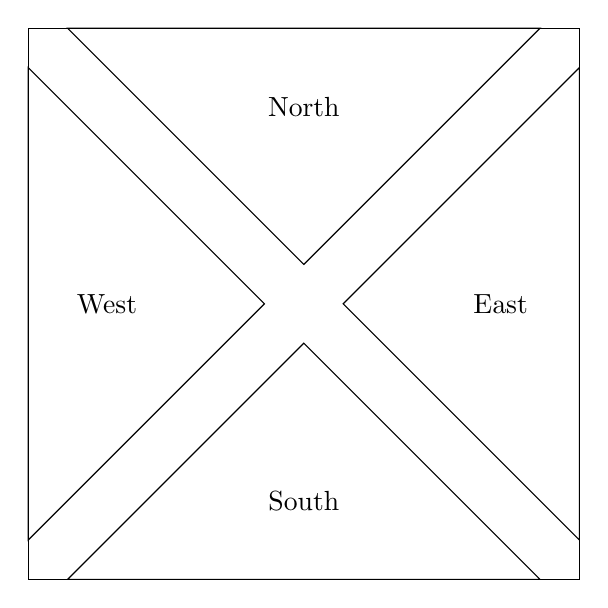
\begin{tikzpicture}[]
            \draw (0,0) -- (7,0) -- (7,7) -- (0,7) -- cycle;
            \draw (0.5,0) -- (6.5,0) -- (3.5,3) -- cycle;
            \draw (7,0.5) -- (7,6.5) -- (4,3.5) -- cycle;
            \draw (6.5,7) -- (0.5,7) -- (3.5,4) -- cycle;
            \draw (0,6.5) -- (0,0.5) -- (3,3.5) -- cycle;
            \node at (6,3.5) {East};
            \node at (3.5,6) {North};
            \node at (1,3.5) {West};
            \node at (3.5,1) {South};
            \end{tikzpicture}
        \end{center}
    \end{figure}
\end{center}


Quantifying the test structures, the location can be referenced by the die position and the quarter (North, East, South and West) on die where the test structures is measured.
There is no recommandations about the metrics for the location.

\subsection{Four-terminal Sensing}

The prefered measurement method for the test structures is the so-calld Four-terminal Sensing, or Kelvin sensing.
This is an electrical impedance measuring technique that uses pairs of current-carrying and voltage-sensing probes to make accurate measurements.

Four-terminal Sensing has advantage for precise measurement of low resistance values by eliminationg the lead and contact resistance for the measurement.
Therefor almost all test structures here using four contact pads to place the probes on them.

%%  ************    LibreSilicon's 1st TestWafer    *******************
%%
%%  Organisation:   Chipforge
%%                  Germany / European Union
%%
%%  Profile:        Chipforge focus on fine System-on-Chip Cores in
%%                  Verilog HDL Code which are easy understandable and
%%                  adjustable. For further information see
%%                          www.chipforge.org
%%                  there are projects from small cores up to PCBs, too.
%%
%%  File:           PearlRiver/Documents/LaTeX/schematic_4terminal.tex
%%
%%  Purpose:        Schematic File for Four-terminal Sensing
%%
%%  ************    LaTeX with circdia.sty package      ***************
%%
%%  ///////////////////////////////////////////////////////////////////
%%
%%  Copyright (c) 2018 by chipforge <hsank@nospam.chipforge.org>
%%  All rights reserved.
%%
%%      This Standard Cell Library is licensed under the Libre Silicon
%%      public license; you can redistribute it and/or modify it under
%%      the terms of the Libre Silicon public license as published by
%%      the Libre Silicon alliance, either version 1 of the License, or
%%      (at your option) any later version.
%%
%%      This design is distributed in the hope that it will be useful,
%%      but WITHOUT ANY WARRANTY; without even the implied warranty of
%%      MERCHANTABILITY or FITNESS FOR A PARTICULAR PURPOSE.
%%      See the Libre Silicon Public License for more details.
%%
%%  ///////////////////////////////////////////////////////////////////
\begin{center}
    Four-terminal Sensing with instrument, probes and device-under-test
    \begin{figure}[h]
        \begin{center}
            \begin{circuitdiagram}{42}{25}
            % current source with ground
            \ground{3}{0}{D}
            \wire{3}{1}{3}{8}
            \othersrc[\modify{RU}]{oo}{3}{11}{V}{}{}
            \wire{3}{14}{3}{21}
            % vertical flow, ampere meter
            \wire{3}{21}{12}{21}
            \measdev[\measunit{A}]{15}{21}{H}{$I_{drive}$}{}
            \wire{18}{21}{24}{21}
            \currarrow{20}{21}{R}{I}
            % pin contact
            \pin[\female]{25}{21}{R}{}
            \pin[\male]{25}{21}{L}{}
            %
            \pin[\female]{25}{1}{R}{}
            \pin[\male]{25}{1}{L}{}
            \ground{24}{0}{D}
            %
            \pin[\female]{25}{6}{R}{}
            \pin[\male]{25}{6}{L}{}
            %
            \pin[\female]{25}{16}{R}{}
            \pin[\male]{25}{16}{L}{}
            % voltage measurement
            \wire{15}{14}{15}{16}
            \wire{15}{16}{24}{16}
            \measdev[\measunit{V}]{15}{11}{V}{$V_{meas}$}{}
            \wire{15}{6}{15}{8}
            \wire{15}{6}{24}{6}
            \Voltarrow{25}{16}{25}{6}{r}{U}
            % device under test
            \resis{40}{11}{V}{DUT}{}
            \wire{26}{1}{35.5}{1}
            \pin{40}{1}{Dr}{}
            \power{35}{1}{R}{I-}
            \wire{26}{6}{35.5}{6}
            \pin{40}{6}{UD}{}
            \power{35}{6}{R}{U-}
            \wire{26}{16}{35.5}{16}
            \pin{40}{16}{UD}{}
            \power{35}{16}{R}{U+}
            \wire{26}{21}{35.5}{21}
            \pin{40}{21}{Ur}{}
            \power{35}{21}{R}{I+}
            %
            \wire{40}{2}{40}{5}
            \wire{40}{7}{40}{8}
            \wire{40}{14}{40}{15}
            \wire{40}{17}{40}{20}
            \end{circuitdiagram}
        \end{center}
    \end{figure}
\end{center}


Best results are given, when the sense wire probes are placed close to device-under-test (DUT) as the inside pair, while the force wire probes are the outside pair.
Otherwise the accuracy can be affected, because more of the lead is included in the measurement.

It is also recommended that every measurement starts with very low current, while voltages could break the test structures.
The current respects the total resistance on the path and results in a voltage which can be measured on the sensing wire probes.
Regarding Ohm's law

\begin{equation}\label{1}
    Resistance = \frac{Voltage}{Current}
\end{equation}

the Resistance can be calculated by driven Current and resulting Voltage.


%%  ************    LibreSilicon's 1st TestWafer    *******************
%%
%%  Organisation:   Chipforge
%%                  Germany / European Union
%%
%%  Profile:        Chipforge focus on fine System-on-Chip Cores in
%%                  Verilog HDL Code which are easy understandable and
%%                  adjustable. For further information see
%%                          www.chipforge.org
%%                  there are projects from small cores up to PCBs, too.
%%
%%  File:           PearlRiver/Documents/LaTeX/die_quarter.tex
%%
%%  Purpose:        Principle Description Pictgure for quarters
%%
%%  ************    LaTeX with circdia.sty package      ***************
%%
%%  ///////////////////////////////////////////////////////////////////
%%
%%  Copyright (c) 2018 by chipforge <hsank@nospam.chipforge.org>
%%  All rights reserved.
%%
%%      This Standard Cell Library is licensed under the Libre Silicon
%%      public license; you can redistribute it and/or modify it under
%%      the terms of the Libre Silicon public license as published by
%%      the Libre Silicon alliance, either version 1 of the License, or
%%      (at your option) any later version.
%%
%%      This design is distributed in the hope that it will be useful,
%%      but WITHOUT ANY WARRANTY; without even the implied warranty of
%%      MERCHANTABILITY or FITNESS FOR A PARTICULAR PURPOSE.
%%      See the Libre Silicon Public License for more details.
%%
%%  ///////////////////////////////////////////////////////////////////
\begin{center}
    Principle - $R_\square$
    \begin{figure}[h]
        \begin{center}
            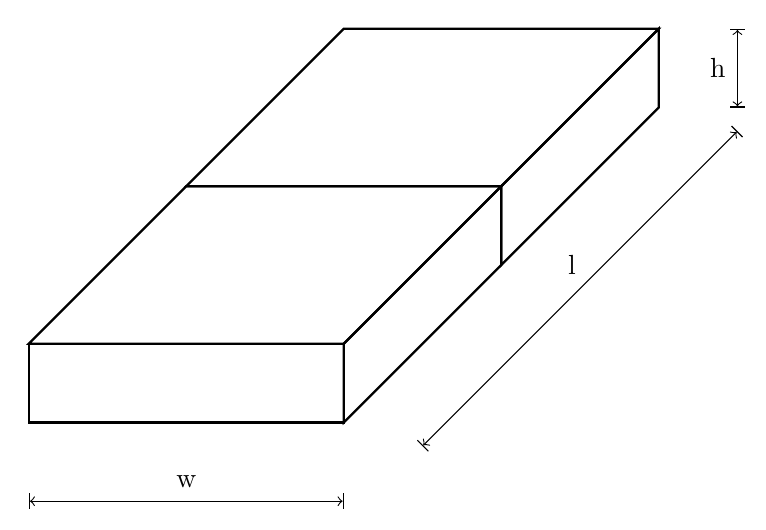
\begin{tikzpicture}[]
            \draw[thick] (0,0) -- (4,0) -- (4,1) -- (0,1) -- cycle; % front
            \draw[thick] (0,1) -- (2,3) -- (6,3) -- (4,1) -- cycle; % 1st top
            \draw[thick] (4,0) -- (4,1) -- (6,3) -- (6,2) -- cycle; % 1st boarder
            \draw[thick] (2,3) -- (4,5) -- (8,5) -- (6,3) -- cycle; % 2nd top
            \draw[thick] (6,3) -- (8,5) -- (8,4) -- (6,2) -- cycle; % 2nd boarder
            % width
            \node at (2,-0.75) {w};
            \draw[|<->|] (0,-1) -- (4,-1);
            % length
            \node at (6.9,2) {l};
            \draw[|<->|] (5,-0.3) -- (9,3.7);
            % hight
            \node at (8.75,4.5) {h};
            \draw[|<->|] (9,4) -- (9,5);
            \end{tikzpicture}
        \end{center}
    \end{figure}
\end{center}


\clearpage
